\section{Review of Graph Neural Networks}
\label{sec:review_of_gnns}

In this section, we formally define the graph neural network (GNN, for short) and briefly survey typical graph neural networks.
We denote a simple graph $\mathcal{G}$ as $\mathcal{G}=(\mathcal{V}, \mathcal{E})$, where $\mathcal{V}$ and $\mathcal{E}$ are the vertex set and the edge set of $\mathcal{G}$, respectively.
Let $n=|\mathcal{V}|$ and $m=|\mathcal{E}|$ as the number of vertices/edges.
We use $v_i$ $(0 \leq i < n)$ to denote a vertex and $e_{i,j}=(v_i, v_j)$ to denote the edge pointing from $v_i$ to $v_j$.
The adjacency set of $v_i$ is $\mathcal{N}(v_i)=\{v|(v_i, v) \in \mathcal{E}\}$.
We denote a \emph{vector} with a bold lower case letter like $\boldsymbol{x}$ and a \emph{matri}x with a bold upper case letter like $\boldsymbol{X}$.

\subsection{General Structure of Graph Neural Networks}

As illustrated in \figurename~\ref{fig:general_structure_of_gnn}, a typical GNN can be decomposed into three parts: an input layer + several GNN layers + a prediction layer.

\begin{figure}
    \centering
    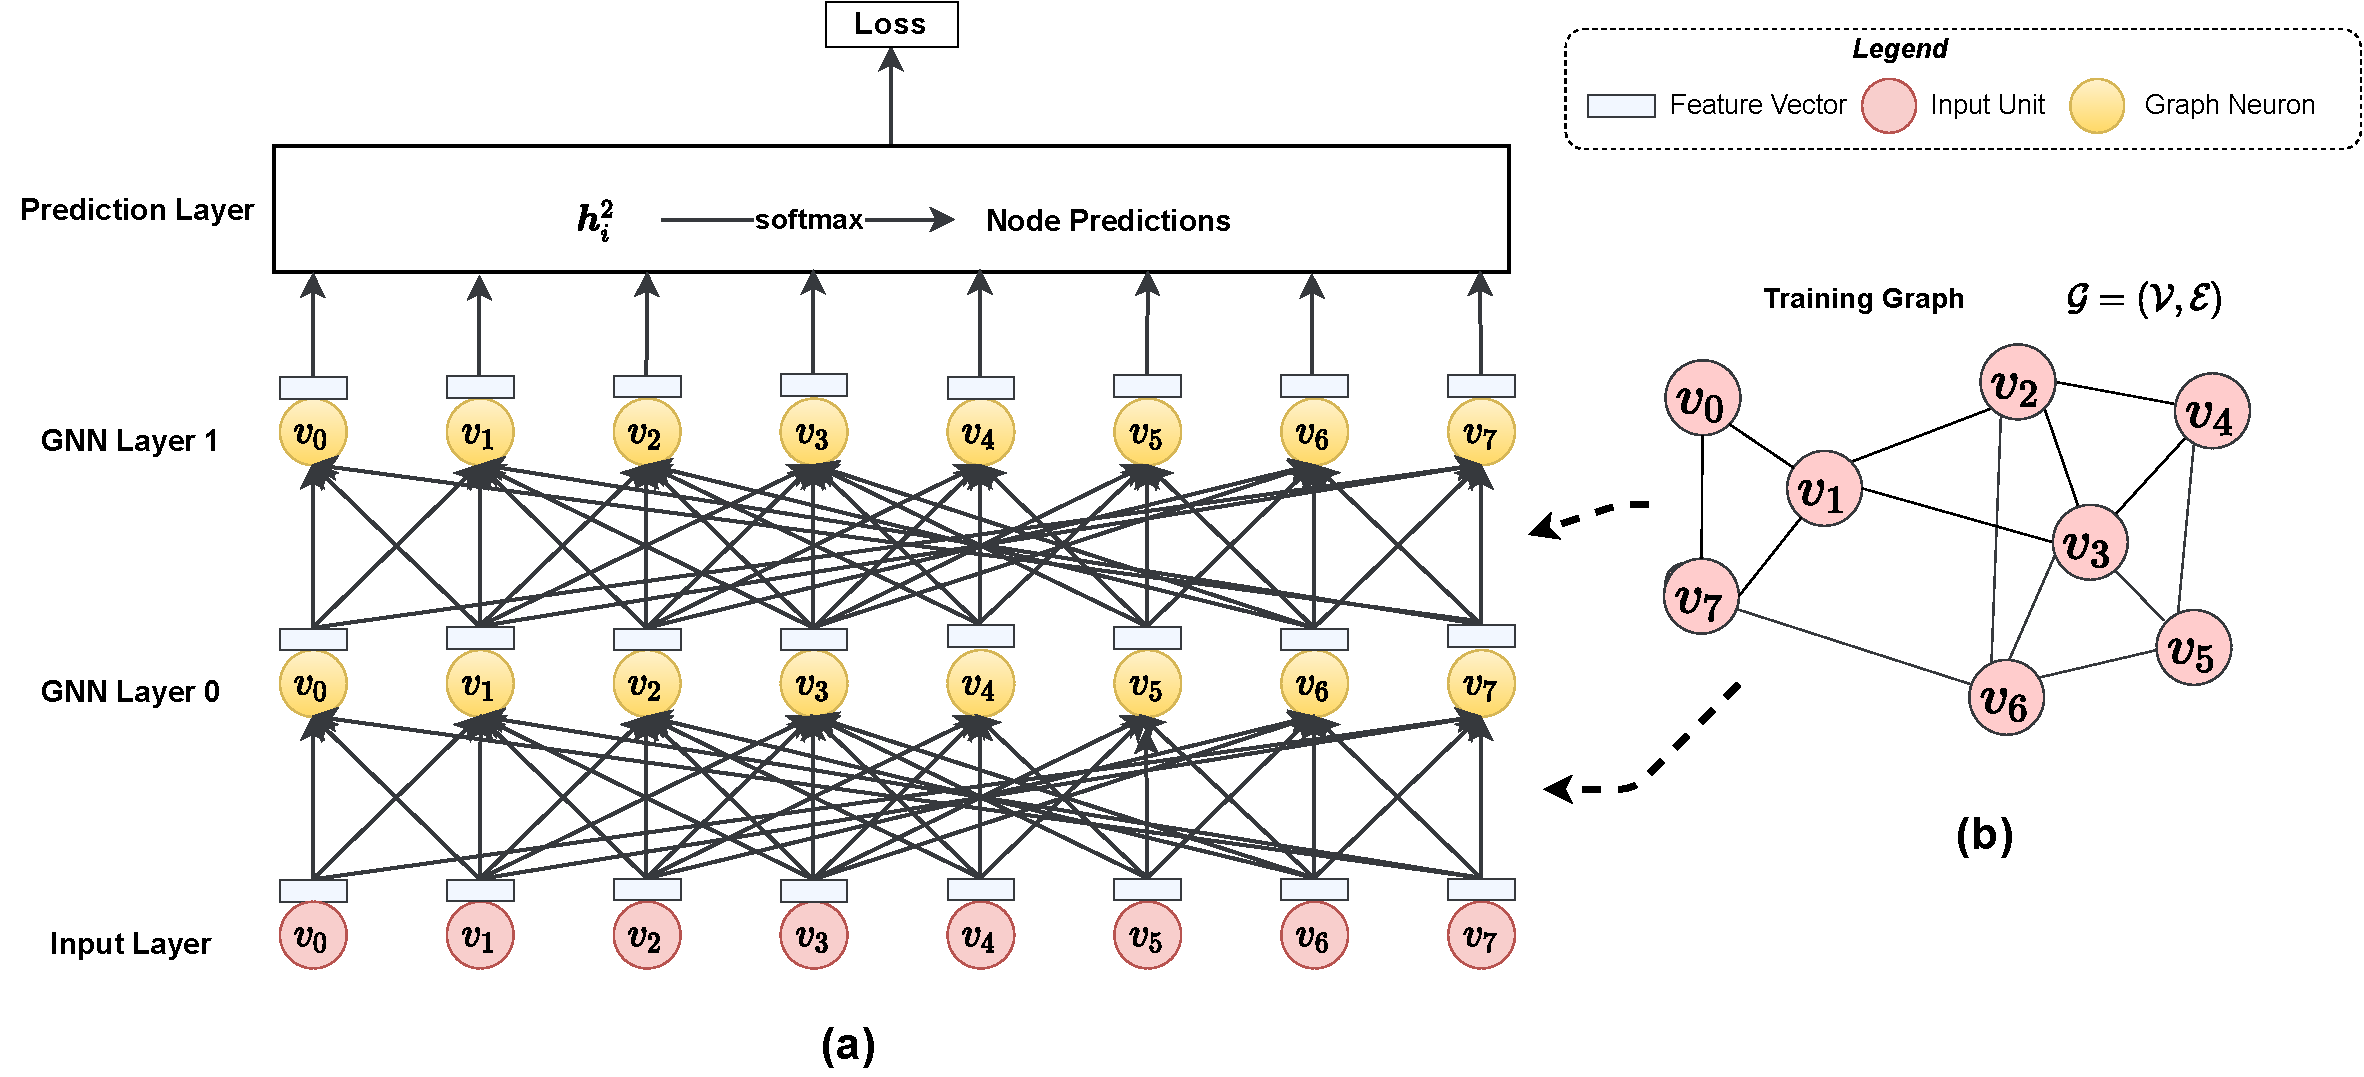
\includegraphics[width=1\columnwidth]{figs/illustration/GNN_common_architecture.pdf}
    \caption{Structure of a typical graph neural network. (a) Demo GNN, (b) Demo graph. The target application is the node classification. The demo GNN has two GNN layers.}
    \label{fig:general_structure_of_gnn}
\end{figure}

A GNN receives a graph $\mathcal{G}$ as the input.
Every vertex $v_i$ in $\mathcal{G}$ is attached with a feature vector $\boldsymbol{x}_i$ to describe the properties of the vertex.
The edges of $\mathcal{G}$ may also be attached with feature vectors $\boldsymbol{e}_{i,j}$
The input layer of a GNN receives feature vectors from all vertices and passes them to GNN layers.

A GNN layer consists of $n$ graph neurons, where $n$ is the number of vertices in $\mathcal{G}$.
Each graph neuron corresponds to a vertex in $\mathcal{G}$.
In the first GNN layer (Layer 0), the graph neuron of the vertex $v_i$ collects input feature vectors of itself and the vertices $\boldsymbol{x}_j$ that are adjacent to $v_i$ in $\mathcal{G}$ (i.e., $v_j \in \mathcal{N}(v_i)$) from the input layer.
After aggregating input feature vectors and applying the non-linear transformation, the graph neuron outputs a hidden feature vector $\boldsymbol{h}^1_i$ for $v_i$.
Take the demo GNN in \figurename~\ref{fig:general_structure_of_gnn}(a) as the example.
Since $\mathcal{N}(v_3) = \{v_1, v_2, v_4, v_5, v_6\}$, the graph neuron of $v_1$ at layer 0 collects the feature vectors \{$\boldsymbol{x}_1$, $\boldsymbol{x}_2$, $\boldsymbol{x}_3$, $\boldsymbol{x}_4$, $\boldsymbol{x}_5$, $\boldsymbol{x}_6$\} from the input layer and outputs $\boldsymbol{h}^1_1$.
Different GNNs mainly differ in the graph neurons that they use.
We elaborate on their details later.

The connection between the input layer and the first GNN layer is determined by the topology of $\mathcal{G}$.
In the traditional neural networks, neurons of neighboring layers are fully connected.
In GNNs, two graph neurons are connected only if their corresponding vertices have an edge between them in $\mathcal{G}$.
Most real-world graphs are very \emph{sparse}, i.e. $|\mathcal{E}| \ll |\mathcal{V}|^2$.


In the next GNN layer (Layer 1), the graph neuron of $v_i$ collects the hidden feature vectors of itself $\boldsymbol{h}^1_i$ and its neighbors ($\boldsymbol{h}^1_j$ with $v_j \in \mathcal{N}(v_i)$) from the \emph{previous} GNN layer.
Based on the collected hidden vectors, the graph neuron in Layer 1 outputs a new hidden feature vector $\boldsymbol{h}^2_i$ for $v_i$.
Though there are only two GNN layers in \figurename~\ref{fig:general_structure_of_gnn}, a GNN allows us to stack more GNN layers to support deeper graph analysis.
%In \figurename~\ref{fig:general_structure_of_gnn}, we shows a GNN with two layers.

Assume there are $L$ GNN layers.
The last GNN layer (Layer $L-1$) outputs a hidden feature vector $\boldsymbol{h}^{L}_i$ for every vertex $v_i$.
As an embedding vector, $\boldsymbol{h}^L_i$ encodes the knowledge learned from the input layer and all the previous GNN layers.
Since $\boldsymbol{h}^L_i$ is affected by $v_i$ and the vertices in the $L$-hop neighborhood of $v_i$, analyzing a graph with a \emph{deeper} GNN means analyzing each vertex with a \emph{wider} scope.

The hidden feature vectors $\boldsymbol{h}^L_i$ of the last GNN layer are fed to the prediction layer to generate the output of the whole GNN.
The prediction layer is a standard neural network.
The structure of the prediction layer depends on the prediction task of the GNN.
Take the node classification task as the example, as shown in \figurename~\ref{fig:general_structure_of_gnn}.
The node classification predicts a label for every vertex in $\mathcal{G}$.
In this case, the prediction layer can be a simple softmax layer with $\boldsymbol{h}^L_i$ as the input and a vector of probabilities as the output.
If the prediction task is edge prediction, the hidden feature vectors of two vertices are concatenated and fed into a softmax layer.
If we need to predict a label for the whole graph, a pooling (max/mean/...) layer is added to generate an embedding vector for the whole graph and the embedding vector is used to produce the final prediction.

Supporting end-to-end training is a prominent advantage of GNN, compared with other graph-based machine learning methods.
We can calculate the gradients of the loss function on the model parameters from the prediction layer directly.
With the help of the backpropagation technique, the gradient is propagated from the prediction layer back to the previous GNN layers layer by layer.
The model parameters are updated with a gradient descent optimizer like Adam.
Except for the input feature vector, there is no need to conduct handworked feature extraction.
In a fully parameterized way, the GNN automatically extracts an embedding vector for each vertex from its $L$-hop neighborhood.
The parameters are tuned according to the specific prediction task, leading to high prediction accuracy.

\subsection{Graph Neuron and Message-passing Model}

Graph neurons are building blocks of a GNN.
A GNN layer consists of $|\mathcal{V}|$ graph neurons.
Each vertex corresponds to a graph neuron.
A graph neuron as shown in \figurename~\ref{fig:graph_neuron_structure} is a small neural network.
The graph neuron of $v_i$ at layer $l$ receives hidden feature vectors $\boldsymbol{h}^l_j$ from the graph neurons of $v_i$ and its neighbors ($v_j \in \{v_i\} \cup \mathcal{N}(v_i)$) at the previous GNN layer \footnote{For the GNN layer 0, graph neurons receive input feature vectors, i.e., $\boldsymbol{h}^0_i=\boldsymbol{x}_i$}.
The graph neuron aggregates the received hidden feature vectors, applies non-linear transformations, and outputs a new hidden feature vector $\boldsymbol{h}_i^{l+1}$.

\begin{figure}
    \centering
    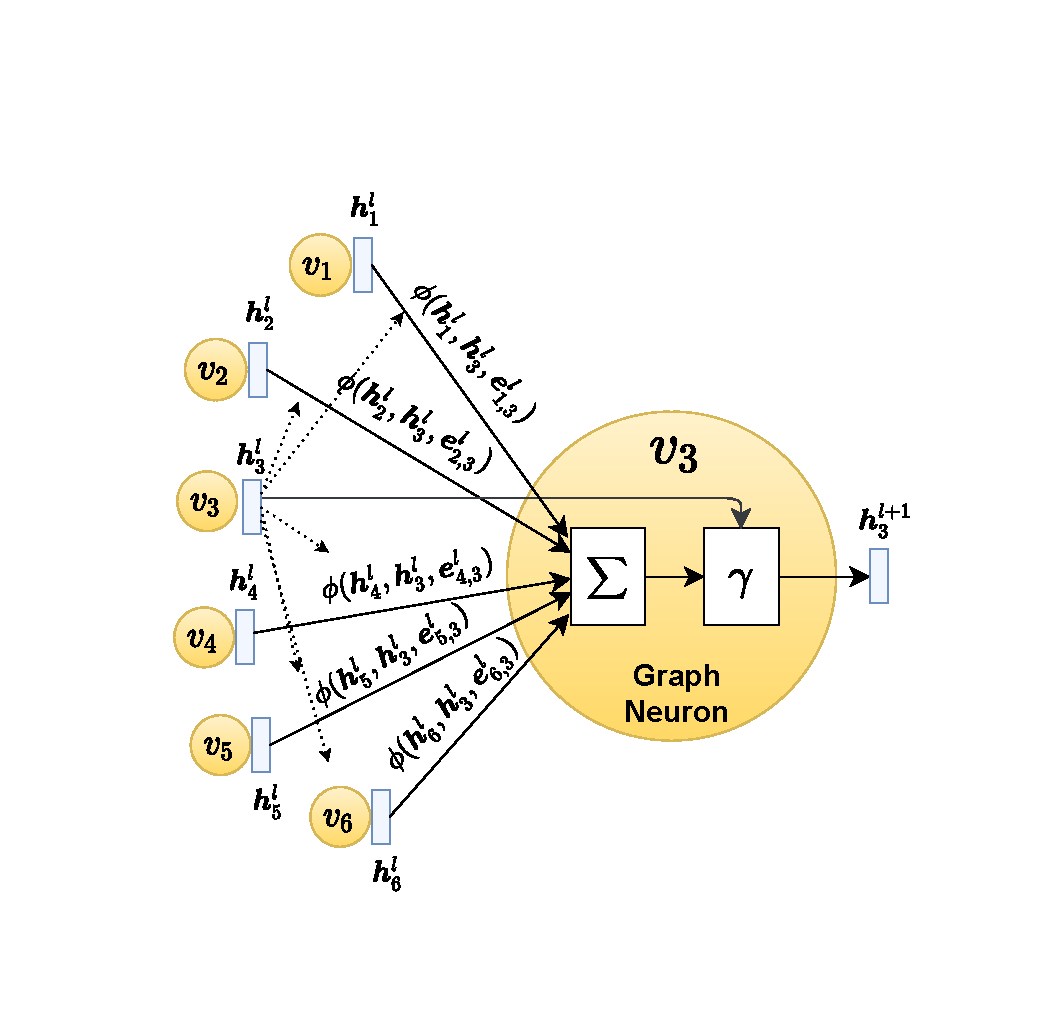
\includegraphics[width=0.5\columnwidth]{figs/illustration/GNN_Unit.pdf}
    \caption{Graph neuron of $v_3$ at the GNN layer $l$ with the graph $\mathcal{G}$ in \figurename~\ref{fig:general_structure_of_gnn}(b). $\phi$/$\Sigma$/$\gamma$ are the message/aggregation/vertex update functions in the message-passing model, respecitvely.}
    \label{fig:graph_neuron_structure}
\end{figure}

We follow the message-passing model \cite{gilmer_messgae_passing} to formally define a graph neuron.
The message-passing model is widely used in the cutting-edge GNN training systems like PyTorch Geometric (PyG) \cite{PyG} and Deep Graph Library (DGL) \cite{DGL}.
\figurename~\ref{fig:graph_neuron_structure} shows the structure of a graph neuron in the message-passing model.
A graph neuron collects messages from its neighbor graph neurons and outputs a hidden feature vector according to the aggregated messages.
Graph neurons at layer $l$ are made of three \emph{differentiable} functions: $\phi^l$, $\Sigma^l$ and $\gamma^l$.
The graph neuron calculates the output hidden vector $\boldsymbol{h}^{l+1}_i$ by
$$
    \boldsymbol{h}^{l+1}_i = \gamma^l(\boldsymbol{h}^l_i, \mathlarger{\Sigma}^l_{v_j \in \mathcal{N}(v_i)}{\phi^l(\boldsymbol{h}^l_i, \boldsymbol{h}^l_j,   \boldsymbol{e}_{j,i})}).
$$

$\phi^l$ is the \emph{message} function.
For every incident edge $(v_j, v_i)$ of $v_i$, $\phi$ receives the output hidden feature vectors $\boldsymbol{h}^l_i$ and $\boldsymbol{h}^l_j$ of the previous GNN layer and the edge feature vector $\boldsymbol{e}_{j,i}$ as the input.
$\phi^l$ emits a message vector $\boldsymbol{m}^l_{j,i}$ for every edge $(v_j, v_i)$ at layer $l$, i.e., $\boldsymbol{m}^l_{j,i}=\phi^l(\boldsymbol{h}^l_i, \boldsymbol{h}^l_j, \boldsymbol{e}_{j,i})$.
For $v_i$, the message vectors $\boldsymbol{m}^l_{x,j}$ of its adjacent edges ($v_x \in \mathcal{N}(v_i)$) are aggregated by the \emph{aggregation} function $\Sigma^l$ to produce an aggregated vector $\boldsymbol{s}^l_i$, i.e., $\boldsymbol{s}^l_i=\mathlarger{\Sigma}^l_{v_j \in \mathcal{N}(v_i)}\boldsymbol{m}^l_{j,i}$.
$v_i$'s aggregated vector $\boldsymbol{s}^l_i$ and its hidden vector $\boldsymbol{h}^l_i$ from the previous GNN layer are fed into the \emph{vertex update} function $\gamma^l$ to calculate the output hidden vector $\boldsymbol{h}^{l+1}_i$ of the current layer $l$, i.e., $\boldsymbol{h}^{l+1}_i = \gamma^l(\boldsymbol{h}^l_i, \boldsymbol{s}^l_i)$
The end-to-end training requires $\phi^l$ and $\gamma^l$ (like multi-layer perceptrons and GRU) and $\Sigma_l$ (like mean, sum, element-wise min/max) are \emph{differentiable} to make the whole GNN differentiable.

Different GNNs adopt different kinds of graph neurons and have different definitions of the three functions.
$\phi$ and $\Sigma$ are the \emph{edge calculation} functions.
They are conducted over every edge in $\mathcal{G}$.
$\gamma$ is the \emph{vertex calculation} function.
It is conducted over every vertex in $\mathcal{G}$.
\tablename~\ref{tab:gnn_overview_edge} and \tablename~\ref{tab:gnn_overview_vertex} list the edge functions and the vertex functions of typical GNNs, respectively.
For ChebNet, we report its GNN sub-layer in the tables.
A ChebNet layer consists of $K$ GNN sub-layers and a summation layer:
$\boldsymbol{H}^{l+1} = \sum_{k=1}^K{\boldsymbol{Z}^{(k)} \textcolor{blue}{\boldsymbol{W}^{(k)}}}$ with the GNN sub-layers $\boldsymbol{Z}^{(1)}=\boldsymbol{H}^l$, $\boldsymbol{Z}^{(2)}=\hat{\boldsymbol{L}}\boldsymbol{H}^l$, and $\boldsymbol{Z}^{(k)}=2\hat{\boldsymbol{L}}\boldsymbol{Z}^{(k-1)} - \boldsymbol{Z}^{(k-2)}$, where $\boldsymbol{H}^l$ is the matrix of output hidden feature vectors of the layer $l-1$.
For GAT, a GAT layer consists of two sub-layers and it conducts part of the vertex calculation before the two sub-layers.
For GaAN, a GaAN layer consists of four sub-layers: the first sub-layer calculates the summation $\boldsymbol{m}_{j, i, (k)}^{l,0}  = \exp((\textcolor{blue}{W^{l, k}_{xa}} \boldsymbol{h}_j^l + \textcolor{blue}{b^{l, k}_{xa}})^T (\textcolor{blue}{\boldsymbol{W}^{l, k}_{ya}} \boldsymbol{h}_i^l + \textcolor{blue}{\boldsymbol{b}^{l,k}_{ya}}))$, and the other three layers calculate $\boldsymbol{m}^l_{j,i,1}$/$\boldsymbol{m}^l_{j,i,2}$/$\boldsymbol{m}^l_{j,i,3}$.

\begin{table}
    \hspace{-5em}
    \begin{footnotesize}
        \begin{tabular}{ccp{8em}p{22em}r}
            \toprule
            GNN                                                                                                                       &
            Type                                                                                                                      &
            $\Sigma$                                                                                                                  &
            $\phi$                                                                                                                    &
            Complexity                                                                                                                  \\ \midrule
            ChebNet \cite{defferrad2016_chebnet}                                                                                      &
            Spectral                                                                                                                  &
            sum                                                                                                                       &
            $\boldsymbol{m}_{j, i}^{(k)} = e_{j, i}\boldsymbol{z}_j^{(k-1)}$                                                          &
            $O(d_{in})$                                                                                                                 \\
            \textbf{GCN} \cite{kipf2017_gcn}                                                                                          &
            Spectral                                                                                                                  &
            sum                                                                                                                       &
            $\boldsymbol{m}_{j, i}^l = e_{j, i} \boldsymbol{h}_j^l$                                                                   &
            $O(d_{in})$                                                                                                                 \\
            AGCN \cite{li2018_agcn}                                                                                                   &
            Spectral                                                                                                                  &
            sum                                                                                                                       &
            $\boldsymbol{m}_{j, i}^l = \tilde{e}_{j, i}^l \boldsymbol{h}_j^l$                                                         &
            $O(d_{in})$                                                                                                                 \\
            GraphSAGE \cite{hamilton2017_graphsage}                                                                                   &
            Non-spectral                                                                                                              &
            mean/LSTM                                                                                                                 &
            $\boldsymbol{m}_{j, i}^l =  \boldsymbol{h}_j^l$                                                                           &
            $O(1)$                                                                                                                      \\
            GraphSAGE-pool \cite{hamilton2017_graphsage}                                                                              &
            Non-spectral                                                                                                              &
            max                                                                                                                       &
            $\boldsymbol{m}_{j, i}^l =  \delta(\textcolor{blue}{\boldsymbol{W}^l_{pool}} \boldsymbol{h}_j^l + \textcolor{blue}{b}^l)$ &
            $O(d_{in} * d_{out})$                                                                                                       \\
            Neural FPs  \cite{duvenaud2015_neural_fps}                                                                                &
            Non-spectral                                                                                                              &
            sum                                                                                                                       &
            $\boldsymbol{m}_{j, i}^l = \boldsymbol{h}_j^l$                                                                            &
            $O(1)$                                                                                                                      \\
            SSE \cite{han2018_sse}                                                                                                    &
            Recurrent                                                                                                                 &
            sum                                                                                                                       &
            $\boldsymbol{m}_{j, i}^l = [\boldsymbol{x}_j \parallel \boldsymbol{h}_j^l]$                                               &
            $O(f+d_{in})$                                                                                                               \\
            \textbf{GGNN}  \cite{li2015_ggnn}                                                                                         &
            Gated                                                                                                                     &
            sum                                                                                                                       &
            $\boldsymbol{m}_{j, i} = \textcolor{blue}{\boldsymbol{W}^l} \boldsymbol{h}_j^l$                                           &
            $O(d_{in} * d_{out})$                                                                                                       \\
            \textbf{GAT}   \cite{huang2018_gat}                                                                                       &
            Attention                                                                                                                 &
            sum                                                                                                                       &
            \begin{scriptsize}
                $\begin{aligned}[t]
                         & \text{Sub-layer 0:}                                                                                                                                                                                    \\
                         & \boldsymbol{m}^{l,0}_{j,i,(k)} = \exp(LeakyReLU(\textcolor{blue}{\boldsymbol{a}^T} [\hat{\boldsymbol{h}}^{l}_{i,(k)} \parallel \hat{\boldsymbol{h}}^{l}_{j, (k)}]))                                    \\
                         & \text{Sub-layer 1:}                                                                                                                                                                                    \\
                         & \alpha^l_{j, i, (k)} = \frac {\exp(LeakyReLU(\textcolor{blue}{\boldsymbol{a}^T} [\hat{\boldsymbol{h}}^{l}_{i,(k)} \parallel \hat{\boldsymbol{h}}^{l}_{j,(k)}] ))} {\hat{\boldsymbol{a}}^{l,0}_{i,(k)}} \\
                         & \text{Multi-head concatenation}: \boldsymbol{m}_{j, i}^{l,1} = \parallel_{k=1}^K \alpha^l_{j, i, (k)} \hat{\boldsymbol{h}}^{l}_{j,(k)}                                                         \\
                         & \text{Multi-head average}: \boldsymbol{m}_{j, i}^{l,1} = \frac{1}{K} \sum_{k=1}^K \alpha^l_{j, i, (k)} \hat{\boldsymbol{h}}^{l}_{j,(k)}
                    \end{aligned}$
            \end{scriptsize}
                                                                                                                                      &
            $
                \begin{aligned}[t]
                    \text{concat: } O(d_{out})      & \\
                    \text{average: } O(K * d_{out}) & \\
                    \text{Two sub-layers}           &
                \end{aligned}
            $
            \\
            \textbf{GaAN}     \cite{zhang2018_gaan}                                                                                   &
            Attention                                                                                                                 &
            sum,max,mean                                                                                                              &
            \begin{scriptsize}
                $\begin{aligned}[t]
                         & \text{Sub-layer 0:}                                                                                                                                                                                                                                                                  \\
                         & \boldsymbol{m}_{j, i, (k)}^{l,0}  = \exp((\textcolor{blue}{W^{l, k}_{xa}} \boldsymbol{h}_j^l + \textcolor{blue}{b^{l, k}_{xa}})^T (\textcolor{blue}{\boldsymbol{W}^{l, k}_{ya}} \boldsymbol{h}_i^l + \textcolor{blue}{\boldsymbol{b}^{l,k}_{ya}}))                                   \\
                         & \text{Sub-layer 1:}                                                                                                                                                                                                                                                                  \\
                         & \alpha^l_{j, i, (k)} = \frac {\exp((\textcolor{blue}{W^{l, k}_{xa}} \boldsymbol{h}_j^l + \textcolor{blue}{b^{l, k}_{xa}})^T (\textcolor{blue}{\boldsymbol{W}^{l, k}_{ya}} \boldsymbol{h}_i^l + \textcolor{blue}{\boldsymbol{b}^{l,k}_{ya}}))} {\hat{\boldsymbol{a}}^{l, 0}_{i, (k)}} \\
                         & \boldsymbol{m}_{j, i}^{l, 1} = \parallel_{k=1}^K \alpha_{j, i, (k)} LeakyReLU(\textcolor{blue}{\boldsymbol{W}^{l, k}_v} \boldsymbol{h}_j^l + \textcolor{blue}{b^{l, k}_v})                                                                                                           \\
                         & \text{Sub-layer 2:}                                                                                                                                                                                                                                                                  \\
                         & \boldsymbol{m}_{j, i}^{l, 2} = \textcolor{blue}{\boldsymbol{W}^l_m} \boldsymbol{h}_j^{l} + \textcolor{blue}{\boldsymbol{b}^l_m}                                                                                                                                                      \\
                         & \text{Sub-layer 3:}                                                                                                                                                                                                                                                                  \\
                         & \boldsymbol{m}_{j, i}^{l, 3} = \boldsymbol{h}_j^l
                    \end{aligned}$
            \end{scriptsize}                                                                                            &
            \makecell[r]{$O(max(d_a, d_m, d_v) * K * d_{in})$                                                                           \\
            Four sub-layers}                                                                                                            \\
            \bottomrule
        \end{tabular}
    \end{footnotesize}
    \caption{Typical graph neural networks and their edge calculation functions.
        $d_{in}$ and $d_{out}$ are dimensions of the input and output hidden feature vectors, respectively.
        Blue variables are model parameters to learn.
    }
    \label{tab:gnn_overview_edge}
\end{table}

\begin{table}
    \begin{footnotesize}
        \begin{tabular}{cp{20em}r}
            \toprule
            GNN                                                                                                                                                                                                              &
            $\gamma$                                                                                                                                                                                                         &
            Complexity                                                                                                                                                                                                         \\ \midrule
            ChebNet \cite{defferrad2016_chebnet}                                                                                                                                                                             &
            $\boldsymbol{z}_i^{(k)} = 2\boldsymbol{s}^{(k)}_{i} - \boldsymbol{z}_i^{(k-2)}$                                                                                                                                  &
            $O(d_{out})$                                                                                                                                                                                                       \\
            \textbf{GCN} \cite{kipf2017_gcn}                                                                                                                                                                                 &
            $\boldsymbol{h}_i^{l+1} = \textcolor{blue}{\boldsymbol{W}}^l  \boldsymbol{s}_i^{l}$                                                                                                                              &
            $O(d_{in} * d_{out})$                                                                                                                                                                                              \\
            AGCN   \cite{li2018_agcn}                                                                                                                                                                                        &
            $\boldsymbol{h}_i^{l+1} = \textcolor{blue}{\boldsymbol{W}}^l  \boldsymbol{s}_i^{l}$                                                                                                                              &
            $O(d_{in} * d_{out})$                                                                                                                                                                                              \\
            GraphSAGE  \cite{hamilton2017_graphsage}                                                                                                                                                                         &
            $\boldsymbol{h}_i^{l+1} =   \delta(\textcolor{blue}{\boldsymbol{W}}^l  [\boldsymbol{s}_i^{l} \parallel \boldsymbol{h}_i^l])$                                                                                     &
            $O(d_{in} * d_{out})$                                                                                                                                                                                              \\
            GraphSAGE-pool   \cite{hamilton2017_graphsage}                                                                                                                                                                   &
            $\boldsymbol{h}_i^{l+1} = \boldsymbol{s}_i^l$                                                                                                                                                                    &
            $O(1)$                                                                                                                                                                                                             \\
            Neural FPs        \cite{duvenaud2015_neural_fps}                                                                                                                                                                 &
            $\boldsymbol{h}_i^{l+1} = \delta(\textcolor{blue}{\boldsymbol{W}}^{l, |\mathcal{N}(i)|}  (\boldsymbol{h}_i^l + \boldsymbol{s}_i^{l}))$                                                                           &
            $O(d_{in} * d_{out})$                                                                                                                                                                                              \\
            SSE             \cite{han2018_sse}                                                                                                                                                                               &
            $\boldsymbol{h}_i^{l+1} = (1 - \alpha)  \boldsymbol{h}_i^l +\alpha    \delta(\textcolor{blue}{\boldsymbol{W}}^l_1 \delta(\textcolor{blue}{\boldsymbol{W}}^l_2 [\boldsymbol{x}_i \parallel \boldsymbol{s}_i^l]))$ &
            $O((f + d_{in}) * d_{out})$                                                                                                                                                                                        \\
            \textbf{GGNN}    \cite{li2015_ggnn}                                                                                                                                                                              &
            \begin{scriptsize}
                $\begin{aligned}[t]
                         & {\boldsymbol{z}}_i^l = \delta ( \textcolor{blue}{\boldsymbol{W}}^z \boldsymbol{s}_i^l + \textcolor{blue}{\boldsymbol{b}}^{sz} + \textcolor{blue}{\boldsymbol{U}}^z \boldsymbol{h}_i^{l} + \textcolor{blue}{\boldsymbol{b}}^{hz})                    \\
                         & \boldsymbol{r}_i^l = \delta ( \textcolor{blue}{\boldsymbol{W}}^r \boldsymbol{s}_i^l+ \textcolor{blue}{\boldsymbol{b}}^{sr} +\textcolor{blue}{\boldsymbol{U}}^r \boldsymbol{h}_i^{l} + \textcolor{blue}{\boldsymbol{b}}^{hr})                        \\
                         & \boldsymbol{h}_i^{l+1} = tanh ( \textcolor{blue}{\boldsymbol{W}} \boldsymbol{s}_i^l + \textcolor{blue}{\boldsymbol{b}}^s + \textcolor{blue}{\boldsymbol{U}} ( \boldsymbol{r}_i^l \odot \boldsymbol{h}_i^{l}) + \textcolor{blue}{\boldsymbol{b}}^h)) \\
                         & \boldsymbol{h}_i^{l+1} = (1 - {\boldsymbol{z}}_i^l) \odot \boldsymbol{h}_i^l + {\boldsymbol{z}}_i^l \odot \boldsymbol{h}_i^{l+1}
                    \end{aligned}$
            \end{scriptsize}
                                                                                                                                                                                                                             &
            $O(d_{in} * d_{out})$                                                                                                                                                                                              \\
            \textbf{GAT} \cite{huang2018_gat}                                                                                                                                                                                &
            \begin{scriptsize}
                $\begin{aligned}[t]
                         & \text{Preprocessing:}                                                                          \\
                         & \hat{\boldsymbol{h}}^{l}_{i,(k)} = \textcolor{blue}{\boldsymbol{W}^{l,k}} \boldsymbol{h}_i^{l} \\
                         & \text{Sub-layer 0:}                                                                            \\
                         & \hat{\boldsymbol{a}}^{l,0}_{i,(k)} = \boldsymbol{s}^{l,0}_{i,(k)}                              \\
                         & \text{Sub-layer 1:}                                                                            \\
                         & \boldsymbol{h}_i^{l+1} = \delta(\boldsymbol{s}_i^{l,1})
                    \end{aligned}
                $
            \end{scriptsize}                                                                                                                                                                                   &
            $
                \begin{aligned}[t]
                    \text{concat:} O(d_{in}*d_{out})    & \\
                    \text{average:} O(K*d_{in}*d_{out}) & \\
                    \text{Two sub-layers}               &
                \end{aligned}
            $
            \\
            \textbf{GaAN}  \cite{zhang2018_gaan}                                                                                                                                                               &
            \begin{scriptsize}
                $\begin{aligned}[t]
                         & \text{Sub-layer 0:}                                                                                                                                                                            \\
                         & \hat{\boldsymbol{a}}^{l,0}_{i,(k)} = \boldsymbol{s}^{l,0}_{i,(k)}                                                                                                                              \\
                         & \text{Sub-layer 1, 2, 3:}                                                                                                                                                                      \\
                         & \boldsymbol{g}_i^l = \textcolor{blue}{\boldsymbol{W}^l_g}[\boldsymbol{h}_i^{l} \parallel \boldsymbol{s}_{i}^{l, 2} \parallel \boldsymbol{s}_{i}^{l, 3}] + \textcolor{blue}{\boldsymbol{b}^l_g} \\
                         & \boldsymbol{h}_i^{l+1} = \textcolor{blue}{\boldsymbol{W}^l_o} [\boldsymbol{h}_i^l \parallel (\boldsymbol{g}_{i}^l \odot \boldsymbol{s}_{i}^{l, 1})] + \textcolor{blue}{\boldsymbol{b}^l_o}
                    \end{aligned}$
            \end{scriptsize}                                                                                                                                                                                   &
            \makecell[r]{$O(max(K * d_v + d_{in}, 2 * d_{in} + d_m) * d_{out})$                                                                                                                                                \\
                Four sub-layers}
            \\ \bottomrule
        \end{tabular}
    \end{footnotesize}
    \caption{Typical graph neural networks and their vertex calculation functions.
        $d_{in}$ and $d_{out}$ are dimensions of the input and output hidden feature vectors, respectively.
        Blue variables are model parameters to learn.
        In Neural FPs, $\textcolor{blue}{\boldsymbol{W}}^{l, |\mathcal{N}(i)|}$ is the weight matrix for vertices with degree $|\mathcal{N}(i)|$ at layer $l$.
    }
    \label{tab:gnn_overview_vertex}
\end{table}

\subsection{Classification of GNNs}

Since we focus on analyzing the performance bottleneck in training GNNs, we classify the typical GNNs from the view of time complexity.
We use $O_\phi$/$O_\Sigma$/$O_\gamma$ to denote the time complexity of the three functions in the message-passing model.
The time complexity of a GNN layer is made up of two parts: the edge calculation complexity $m * (O_\phi$ + $O_\Sigma)$ and the vertex calculation complexity $n * O_\gamma$.

In \tablename~\ref{tab:gnn_overview_edge} and \tablename~\ref{tab:gnn_overview_vertex}, we list the edge and vertex calculation complexity, respectively.
The time complexity of a graph neuron is affected by the dimensions of the input/output hidden vectors $d_{in}$ and $d_{out}$ and the dimensions of the model parameters (like the number of heads $K$ in GAT and the dimensions of the view vectors $d_a$/$d_v$ in GaAN).

We classify the typical GNNs into four quadrants based on their edge/vertex complexity as shown in \figurename~\ref{fig:gnn_complexity_quadrant}. We pick GCN, GGNN, GAT, and GaAN as the \emph{representative GNNs} of the four quadrants.

\begin{figure}
    \centering
    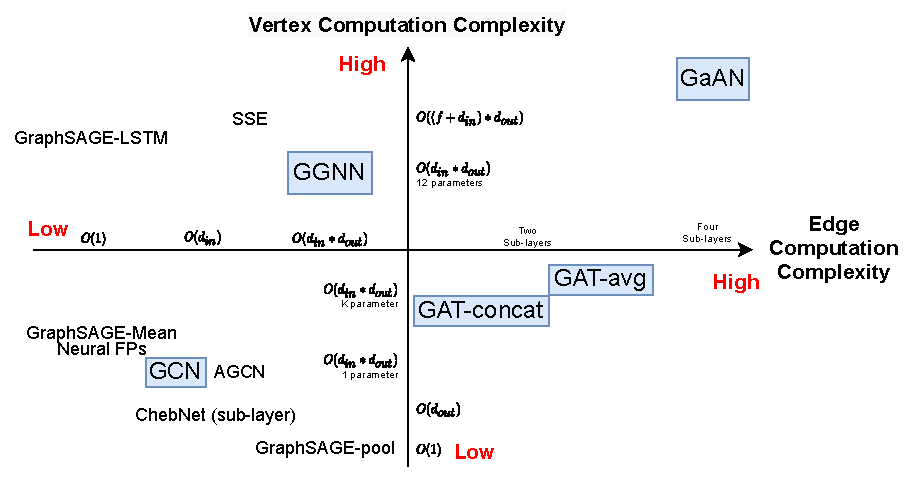
\includegraphics[width=0.7\columnwidth]{figs/illustration/GNN_complexity_quadrant.pdf}
    \caption{Complexity quadrants of typical GNNs. We compare the complexity according to the number of sub-layers, the Big-O notation and the number of parameters to train.}
    \label{fig:gnn_complexity_quadrant}
\end{figure}

\textbf{GCN} \cite{kipf2017_gcn} (low vertex \& edge calculation complexity): Graph convolution network (GCN) is the first-order approximation of the spectral-based graph convolutions.
%By combining the advantages of both the spectral-based and the spatial-based convolution, it can learn the representation of the local topological structure and vertex features efficiently.
It has only one parameter to learn at each layer, i.e. the weight matrix $\boldsymbol{W}^l$ in $\gamma$.
A GCN graph neuron can be expressed as $\boldsymbol{h}^{l+1}_i = \boldsymbol{W}^l\sum_{v_j \in \mathcal{N}(v_i)}{e_{j,i}\boldsymbol{h}^l_j}$, where $e_{j,i}$ is the normalized weight of the edge $(v_j, v_i)$.
%In the matrix view, $\boldsymbol{H}^{l+1} = (\boldsymbol{A}\boldsymbol{H}^l)\boldsymbol{W}^l$.
According to the associative law of the matrix multiplication, $\boldsymbol{h}^{l+1}_i = \sum_{v_j \in \mathcal{N}(v_i)}{e_{j,i}\boldsymbol{W}^l\boldsymbol{h}^l_j}$.
Since the dimension of $\boldsymbol{h}^{l+1}_i$ is usually smaller than $\boldsymbol{h}^l_i$ in practical GCNs, the implementation of GCN in PyTorch Geometric chooses to first conduct the vertex calculation $\hat{\boldsymbol{h}}^l_j = \boldsymbol{W}^l\boldsymbol{h}^l_j$ for each vertex $v_j$ and then conduct the edge calculation $\boldsymbol{h}^{l+1}_i=\sum_{v_j\in\mathcal{N}(v_i)}{e_{j,i}\hat{\boldsymbol{h}}^l_j}$.
As $\hat{\boldsymbol{h}}^l_j$ has the same dimension as $\boldsymbol{h}^{l+1}_i$, the implementation significantly reduces the  computation cost of the edge calculation.

\textbf{GGNN} (high vertex \& low edge calculation complexity):
GGNN introduces the gated recurrent unit (GRU) into the graph neural networks.
The vertex update function $\phi$ of GGNN is a modified GRU unit that has 12 model parameters to learn, having high computational complexity.
To lower the training cost, all GNN layers share the same group of parameters in GGNN.
GGNN further requires the dimension of $\boldsymbol{h}^{l+1}$ is equal to the dimension of $\boldsymbol{h}^l$.
Since the message function $\phi$ only uses the hidden feature vector $\boldsymbol{h}^l_j$ of the source vertex $v_j$ of an edge $(v_j, v_i)$, in the implementation, GGNN conducts the pre-processing vertex calculation $\hat{\boldsymbol{h}}^l_i=\boldsymbol{W}\boldsymbol{h}^l_i$ for every vertex $v_i$ before the message-passing.
The message function $\phi$ directly uses $\hat{\boldsymbol{h}}^l_j$ as the message vector for the edge $(v_j, v_i)$.
In this way, GGNN further reduces the time complexity of the edge calculation to $O(1)$ without increasing the time complexity of the vertex calculation.

\textbf{GAT} (low vertex \& high edge calculation complexity):
GAT introduces the attention and multi-head mechanism into the graph neural networks.
The $K$ heads generate $K$ independent views for an edge, where $K$ is a hyper-parameter.
The views of $K$ heads can be merged by concatenating or by averaging.
For concatenating, the dimension of the hidden feature vector of each head $d_{head}$ is $d_{out}/K$.
For averaging, $d_{head}$ is $d_{out}$, multiplying the complexity by $K$.
Each GAT layer consists of a preprocessing step and two sub-layers.
In the preprocessing step, GAT calculates the attention vectors $\hat{\boldsymbol{h}}^{l}_{i,(k)}$ for every vertex $v_i$ in every head $k$.
The first sub-layer uses the attention vectors to calculate the attention weights of every edge in every head $\boldsymbol{m}^{l,0}_{j,i,(k)}$.
After the message-passing, the first-layer gets the summation of attention weights of every vertex in every head $\hat{\boldsymbol{a}}^{l,0}_{i,(k)}$.
The second sub-layer gets the normalized attention weights $\alpha_{j, i, (k)}$ for every edge in every head and aggregates the hidden feature vectors with the normalized weights in the message-passing.
GAT uses the aggregated vector $\boldsymbol{s}^{l,1}_i$ of the second sub-layer as the output hidden vector directly.

\textbf{GaAN} (high vertex \& edge calculation complexity):
Based on the multi-head mechanism, GaAN introduces a convolutional subnetwork to control the weight of each head. Different from to multi-head mechanism in GAT, GaAN project the center vertex feature to the query vector (dimension is $d_v$), and
the neighboring vertex features are projected to get key and value vectors. The dimension of key and values vectors are the same, we set to $d_a$.
$K$ is the number of attention heads. The weight of each head is calculated by a convolutional network, which takes the feature of each vertex and its neighbors as input to get the gated values with a dimension of $K$.
The convolutional network is built by combining average pooling and max pooling. Moreover, the max-pooling needs to project the vertex feature to a transformed vector with a dimension of $d_m$, costing an additional computational overhead.
Each GaAN layer consists of four sub-layers. The first sub-layer aims to get the summation of attention weights of every vertex in each head.
The second sub-layer uses to aggregate neighboring vertices' query vector with the normalized attention weights $\alpha_{j, i, (k)}$ for every head.
And the third sub-layer is used in max-pooling and it gets the element-wise max vector of neighboring vertices' transformed vectors by message-passing.
The last sub-layer gets element-wise mean vector of neighboring vertices' vectors by message-passing. The gate values $\boldsymbol{g}^l_i$ is obtained by using a fully-connected layer with vector concatenating $\boldsymbol{h}^{l}_i$, $\boldsymbol{s}^{l, 2}_i$ and $\boldsymbol{s}^{l, 3}_i$.
At last, GaAN uses a fully-connected layer with concatenating $\boldsymbol{h}^{l}_i$ and the result of element-wise multiplying $\boldsymbol{g}^{l}_i$ and $\boldsymbol{s}^{l, 0}_i$ to get the output hidden vector.

\subsection{Sampling Techniques}

By default, GNNs are trained in a full-batch way, using the whole graph in each iteration.
The full-batch gradient descent has two disadvantages \cite{chiang2019_cluster_gcn}.
It has to cache intermediate results of all vertices in the forward phase, which consumes lots of memory space.
It updates the parameters only once for each epoch, slowing the convergence of gradient descent.

To train GNNs in a mini-batch way, several sampling techniques are proposed.
In each mini-batch, they sample a small subgraph from the whole graph $\mathcal{G}$ and uses the subgraph to update the model parameters.
In other words, the sampling techniques only active the graph neurons and the connections that appear in the sampled subgraph between GNN layers, as shown in \figurename~\ref{fig:gnn_sampling}.
Inactive graph neurons and connections do not participate in the training of this mini-batch, saving lots of computation and storage costs.
Moreover, it may reduce the risk of overfitting the training graph.
Based on whether different GNN layers sample different subgraphs, the existing sampling techniques can be divided into two groups \cite{zeng2020_graphsaint}: the neighbor sampling and the graph sampling.

The neighbor sampling techniques \cite{hamilton2017_graphsage, ying2018_pinsage, chen2018_fastgcn, chen2018_sgcn, huang2018_adap} sample the subgraphs layer by layer.
The first sample several vertices from $\mathcal{V}$ in the last GNN layer.
Then they repeatedly sample the neighbors of those vertices in the previous layer until the input layer.
The sampled subgraphs of different GNN layers may be \emph{different}, as shown in \figurename~\ref{fig:gnn_sampling_neighbor_sampling}.
GraphSAGE \cite{hamilton2017_graphsage} is the representative technique.
For every sampled vertex $v_i$ in the GNN layer $l$, GraphSAGE samples at most $S^l$ neighbors of $v_i$ in the previous GNN layer.
$S^l$ is the hyperparameter that is usually much smaller than $|\mathcal{V}|$.
In this way, GraphSAGE limits the neighborhood sizes of the vertices in the sampled subgraph, especially high-degree vertices.

\begin{figure}
    \centering
    \subfloat[Neighbor sampling\label{fig:gnn_sampling_neighbor_sampling}]{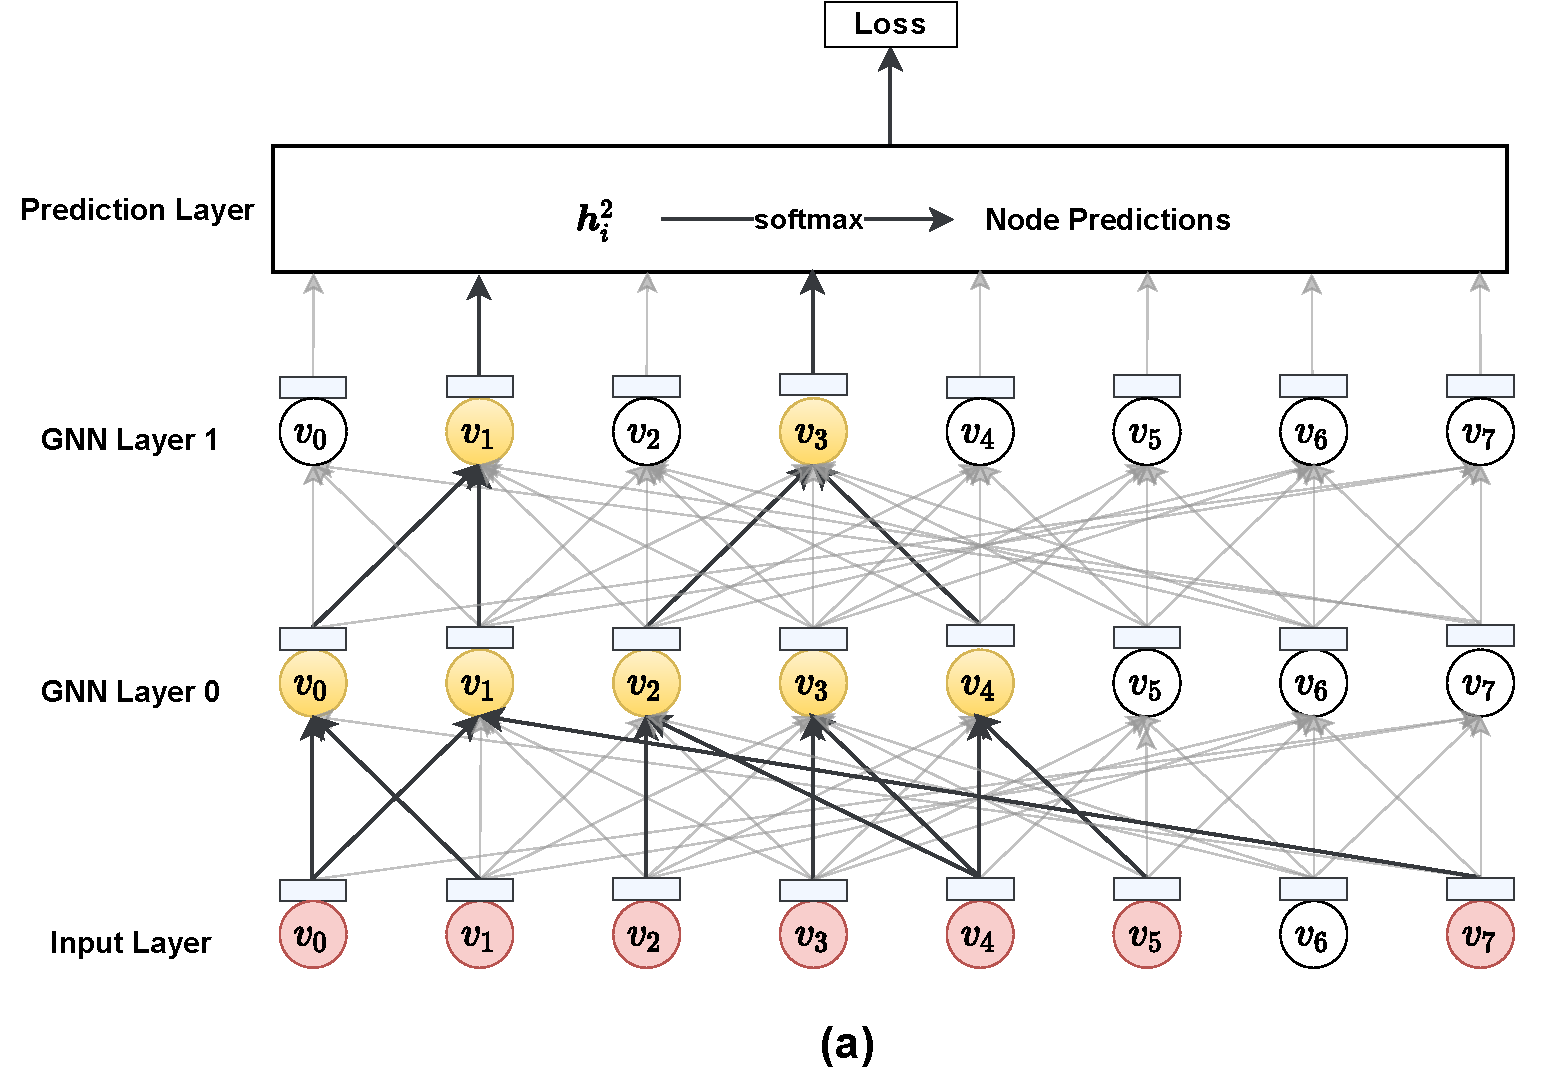
\includegraphics[height=4.1cm]{figs/illustration/layer_sampling.pdf}}
    %
    \subfloat[Graph sampling\label{fig:gnn_sampling_graph_sampling}]{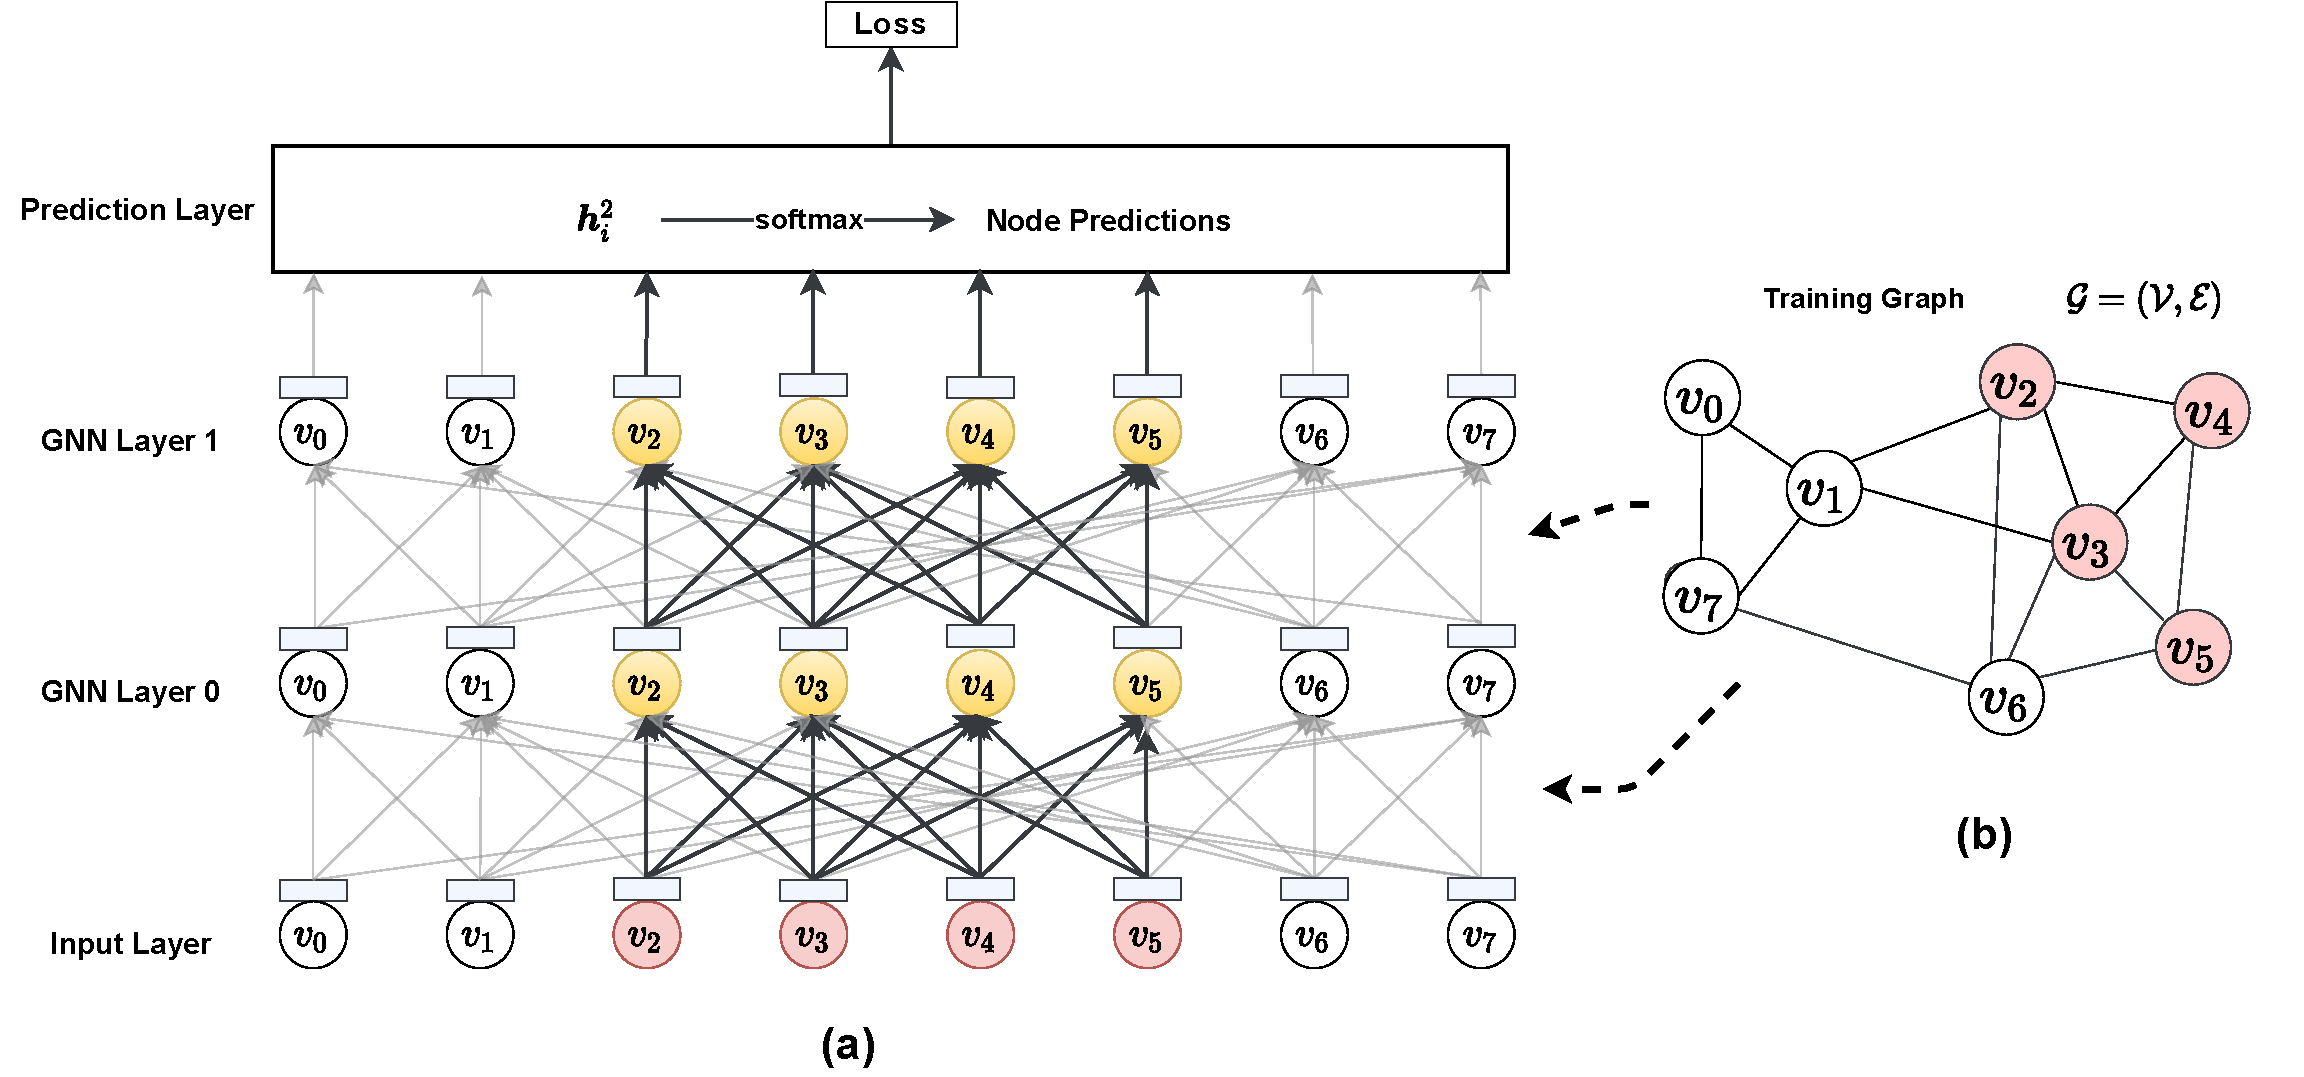
\includegraphics[height=4.1cm]{figs/illustration/graph_sampling.pdf}}
    \caption{Training a GNN with sampling techniques. The faded graph neurons and their connections are inactivated.}
    \label{fig:gnn_sampling}
\end{figure}

The graph sampling techniques \cite{zeng2018_aesg, chiang2019_cluster_gcn, zeng2020_graphsaint} sample a subgraph for each mini-batch and use the same sampled graph for all GNN layers, as shown in \figurename~\ref{fig:gnn_sampling_graph_sampling}.
They differ in the methods to sample subgraphs.
The cluster sampler technique \cite{chiang2019_cluster_gcn} is the representative technique.
Given a training graph $\mathcal{G}$, it partitions $\mathcal{G}$ into closely connected clusters.
For each mini-batch, it randomly picks $K$ clusters, where $K$ is the hyperparameter.
The technique ignores the inter-cluster edges and only keeps the intra-cluster edges in the subgraph.


